\documentclass[12pt]{article}
\setlength{\oddsidemargin}{0in}
\setlength{\evensidemargin}{0in}
\setlength{\textwidth}{6.5in}
\setlength{\parindent}{0in}
\setlength{\parskip}{\baselineskip}
\usepackage{amsmath,amsfonts,amssymb}
\usepackage{graphicx}
\usepackage{enumitem}
\usepackage[]{algorithmicx}
\usepackage{amsthm}
\usepackage{fancyhdr}
\pagestyle{fancy}
\setlength{\headsep}{36pt}
\usepackage{tkz-berge}
\usetikzlibrary{positioning, automata}

\usepackage{hyperref}

\theoremstyle{remark}
\newtheorem*{solution}{Solution}

\newcommand{\makenonemptybox}[2]{%
%\par\nobreak\vspace{\ht\strutbox}\noindent
\item[]
\fbox{% added -2\fboxrule to specified width to avoid overfull hboxes
% and removed the -2\fboxsep from height specification (image not updated)
% because in MWE 2cm is should be height of contents excluding sep and frame
\parbox[c][#1][t]{\dimexpr\linewidth-2\fboxsep-2\fboxrule}{
  \hrule width \hsize height 0pt
  #2
 }%
}%
\par\vspace{\ht\strutbox}
}
\makeatother

\begin{document}
\definecolor {processblue}{cmyk}{0.96,0,0,0}

\lhead{{\bf CSCI 3104, Algorithms \\ Problem Set 6a (10 points)} }
\rhead{Name: \fbox{Michael Rogers} \\ ID: \fbox{105667404} \\ {\bf Profs.\ Hoenigman \& Agrawal\\ Fall 2019, CU-Boulder}}
\renewcommand{\headrulewidth}{0.5pt}

\phantom{Test}

\begin{small}
\textbf{Instructions for submitting your solution}:
\vspace{-5mm} 

\begin{itemize}
	\item The solutions \textbf{should be typed} and we cannot accept hand-written solutions. \href{http://ece.uprm.edu/~caceros/latex/introduction.pdf}{Here's a short intro to Latex.}
	\item You should submit your work through \href{https://www.gradescope.com/courses/59294}{\textbf{Gradescope}} only.
	\item If you don't have an account on it, sign up for one using your CU email. You should have gotten an email to sign up. If your name based CU email doesn't work, try the identikey@colorado.edu version. 
	\item Gradescope will only accept \textbf{.pdf} files (except for code files that should be submitted separately on Gradescope if a problem set has them) and \textbf{try to fit your work in the box provided}. 
	\item You cannot submit a pdf which has less pages than what we provided you as Gradescope won't allow it. 
	\item Verbal reasoning is typically insufficient for full credit. Instead, write a logical argument, in the style of a mathematical proof.
	\item For every problem in this class, you must justify your answer:\ show how you arrived at it and why it is correct. If there are assumptions you need to make along the way, state those clearly.
	
	\item You may work with other students. However, \textbf{all solutions must be written independently and in your own words.} Referencing solutions of any sort is strictly prohibited. You must explicitly cite any sources, as well as any collaborators. 
\end{itemize}



\vspace{-4mm} 
\end{small}

\hrulefill

\newpage
\begin{enumerate}
\item (1 pt) What do the edge weights of a graph $G$ in a maximum-flow network represent?

\begin{solution}
Capacity
\end{solution}

\item (2 pts) What are the two conditions that must be met for network flow?
\begin{solution}
Capacity - $\forall$ e $\in$ E, for some graph $G=(V,E)$, $0\leq f(e) \leq c(e)$ \\ \\ 
Conservation - $\forall$ v $\in$ V, for some graph $G=(V,E)$, $$\sum_{\text{e into v}} f(e) = \sum_{\text{e out of v}} f(e)$$
\end{solution}


\item (2 pts) What do the edge weights in the residual graph $G_f$ represent? Include both forward and backward edges.
\begin{solution}
Forward Edges - Forward edges represent the amount of remaining units of flow that can be pushed through that edge.\\ \\
Backward Edges- Represent the amount of flow that can be pushed back to a vertex in a given edge.
\end{solution}

\pagebreak
\item (5 pts) Based on the following network and the given edge capacities answer the following. 
\begin{figure}[h!]
\begin{center}
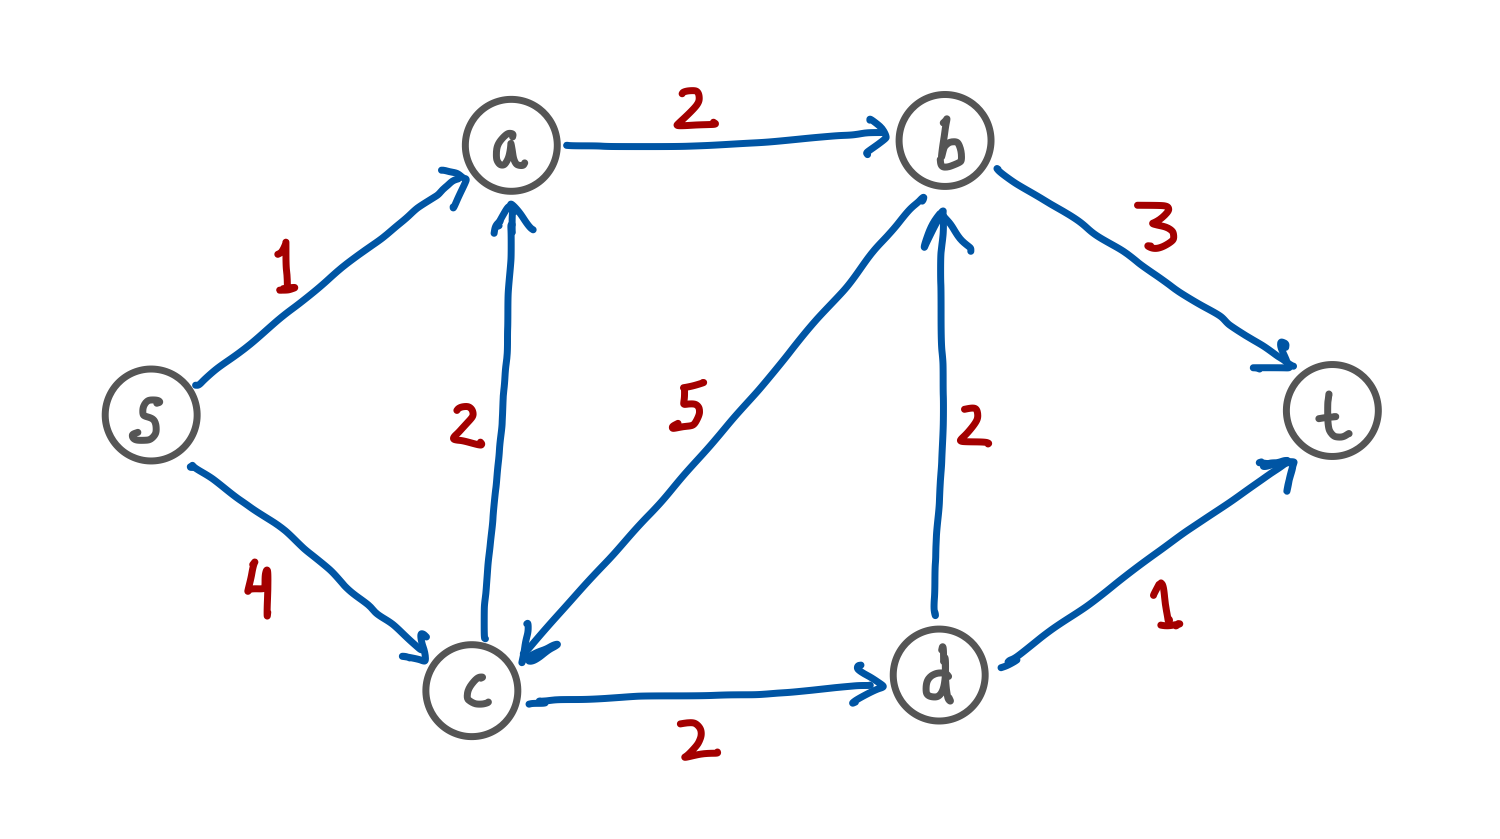
\includegraphics[scale=0.3]{Flow_6a.jpeg}
\end{center}
\end{figure}

\begin{enumerate}
\item (1 pts) Can the max flow be 5 (capacity($e_{sa}$) + capacity($e_{sc}$))? Justify your answer in one sentence.
\begin{solution}
No, becuase the max flow capacity that can go into $t$ is 4 and since \\flow $\geq$ capacity, it cannot be possible.
\end{solution}

\item (2 pts) For the graph, identify one simple $s-t$ path and the bottleneck edge value on that path. Also report the maximum allowed flow on this $s-t$ path.
\begin{solution}
For the path $s-a-b-t$ the bottleneck value is 1 which comes from edge $s-a$. The max flow on this path is 1 because if it were bigger then \\flow $\geq$ capacity for $s-a$.
\end{solution}

\item (2 pts) Assuming all $f(e)$ are initially 0 where $f$ represents flow, what are the residual capacities on the forward and backward edges of $G_f$ after one iteration of the Ford-Fulkerson algorithm. Use the simple path you identified in Part b. 
\begin{solution} Residual Values: \\
$s-a$ = 0, $(s-a)'$ = 1 \\ 
$a-b$ = 1, $(a-b)'$ = 1 \\ 
$b-t$ = 1, $(b-t)'$ = 2 \\ 
\\ All other edges are still set to 0
\end{solution}

\end{enumerate}
\end{enumerate}


\end{document}